\documentclass[conference]{IEEEtran}
\IEEEoverridecommandlockouts
% The preceding line is only needed to identify funding in the first footnote. If that is unneeded, please comment it out.
\usepackage{cite}
\usepackage{amsmath,amssymb,amsfonts}
\usepackage{algorithmic}
\usepackage{graphicx}
\usepackage{textcomp}
\usepackage{xcolor}


% \setlength{\parindent}{4em}
\setlength{\parskip}{0.5em}

\def\BibTeX{{\rm B\kern-.05em{\sc i\kern-.025em b}\kern-.08em
    T\kern-.1667em\lower.7ex\hbox{E}\kern-.125emX}}
\begin{document}

\title{A Convolutional Neural Network to Diagnose Pneumonia from Frontal Chest X-Ray Images\\
}

\author{\IEEEauthorblockN{Kevin Mao}
\IEEEauthorblockA{\textit{Columbia University, Computer Science} \\
New York City, NY \\
kevin.mao@columbia.edu}
\and
\IEEEauthorblockN{Alex Kim}
\IEEEauthorblockA{\textit{Columbia University, Biomedical Engineering} \\
New York City, NY \\
agk2144@columbia.edu}
}

\maketitle

\begin{abstract}
Pneumonia is the leading cause of death among children under 5 years old \cite{unicef}, and early diagnosis in critical for proper treatment. In this paper, we show that transfer learning applied to large convolutional neural networks can be used to diagnose pneumonia using a Kaggle dataset of 5,858 frontal chest X-ray images \cite{kaggle} from 5,232 unique children. We were able to replicate previous work and build on this by developing a multi-class model that could differentiate viral and bacterial pneumonia

We developed two models, for differentiating between (1) normal and infected images, and (2) normal, bacterial, and viral pneumonia images. Our binary algorithm achieved a best F1 test score of 0.941 and accuracy 91.441\% with three hidden layers, batch size of 64, learning rate of 0.001, and 50 epochs. This performance was within a similar range as previous work with this dataset \cite{kermany2018identifying}. Our multi-classifying algorithm achieved a best F1 test score of 0.636 and accuracy 83.784\% with three hidden layers, batch size of 1000, learning rate of 0.001, and 400 epochs.

We have shown that our model is capable of binary and 3-class classification of chest X-ray images for pneumonia, but more can be done to further improve performance.

\end{abstract}

\begin{IEEEkeywords}
Convolutional Neural Network, Pneumonia, Chest X-Ray, Biosignals, Deep Learning
\end{IEEEkeywords}

\section{Introduction}
According to a study done by UNICEF, pneumonia remains the leading cause of death among children under 5 years old \cite{unicef}. In 2015, pneumonia was responsible for 922,000 child deaths, making up almost 16\% of all child deaths \cite{cdc}. More than 1 million people in the US alone are hospitalized from pneumonia every year \cite{cdc}. Despite there being effective methods to diagnose and treat pneumonia, high poverty areas with suboptimal health conditions (malnutrition, contaminated water and air pollution) are greatly affected by the disease \cite{unicef}. 

Pneumonia arises when inflammation occurs in the alveoli of lungs due to the presence of bacteria or viruses. These contaminants can be introduced via water droplets or food particles that enter the respiratory tract \cite{pneumoniaoverview}. While healthy adults can recover fairly quickly, for younger and older patients with weakened immune systems pneumonia may be life threatening. 

Methods of diagnosing pneumonia may range depending on the resources available. Diagnoses in low-income countries primarily rely on identifying symptoms early with simple clinical procedures, such as observing the breathing quality and rate of the patient using a stethoscope. Patients with access to more precise methods may have an x-ray of their lungs taken to identify which part of the lung tissue is inflamed \cite{pneumoniaoverview}.  

There are several issues that remain with the status quo of radiology exams. A combination of low resources and high volume may lead to misclassifications and consequent misdiagnoses by WHO protocol trained radiologists. In fact, studies have shown there are discrepancies in the assessment of radiographs between radiologists (with concordance rates between two reviewers to be as low as 48\%) \cite{plos}. Secondly, proper treatment of pneumonia depends on the correct identification of the pathogen. Antibiotics, like amoxicillin, are administered as a blanket drug for children pneumonia diagnoses in low-income regions, which may not be effective against viral pneumonia or other forms of bacteria with different site specificities.

Artificial intelligence has shown promise in surpassing the performance of medical professionals for classification tasks. Traditional methods of image analysis involved a triad approach of manually segmenting objects of interest, developing classifiers for each class of objects, and classifying the image \cite{ieee}. Now, convolutional neural networks have become a standard architecture for processing and classifying images. Deep neural networks have shown an ability to quantify features that are indicative of the diseases like diabetes mellitus (from retinopathy images) \cite{retinopathy} and skin cancer (from images of skin) with high accuracy \cite{skincancer}. 

For this study, we adopted a transfer learning approach which involves reusing a base network trained on a base dataset and repurposing the learned features to a dataset of interest. This process is made possible as deep NN’s that are trained on images tend to learn similar features. The weights of this model learned on extremely large datasets like the Stanford ImageNet dataset can be leveraged and retrained on the last layer with back-propagation to recognize shared features in biomedical images like chest x-rays. In this project, we explore a transfer learning framework using Google’s ImageNet model to effectively classify normal, viral, and bacterial pneumonia in pediatric chest X-rays images.
\section{Materials and Methods}

\subsection{Problem Formulation}

For the purposes of this experiment, two problems were considered. Given the nature of the dataset which was divided into normal and abnormal (bacterial and viral separately labelled) pneumonia images we decided to assess the performance of the network as both a binary (normal vs. abnormal) and multi label classifying (normal vs. bacterial vs. viral) problem. Input X is the provided chest X-ray images and the output Y is a label $y\in\{0,1\}$ for the binary classifier and $y \in \{0,1,2\}$ for the multi-classifier. A binary cross entropy loss function was optimized for the binary classifier, and a sparse softmax cross entropy (categorical cross entropy loss) for the multi-classifer.

In order to combat potentially dangerous misdiagnoses, precision and recall performance metrics can be used to give false negatives higher costs than false positives. The F1-score accounts for both precision and recall scores, and is used to gauge the performance of our network. Accuracy is also recorded.

\subsection{Model Architecture and Training}
We used large convolutional neural networks that were pre-trained on the ImageNet dataset and switched out their last classification layers for ours. We tried both Xception and InceptionV3 models, models that had been used in previous studies \cite{retinopathy} \cite{kermany2018identifying}, but found better results with Inception. After the pretrained model, we added a global average pooling layer, followed by a variable number of dense layers. The output after the global average pooling layer was saved and loaded in a separate model comprised only of dense layers, and this was the model we trained. This technique significantly sped up training times without sacrificing performance. We used an Adam Optimizer for training and found the best number of epochs, batch size, and training step empirically. Training was done on Google Cloud Deep Learning VM with a NVIDIA Tesla V100 GPU and all code was written in Tensorflow. Figures 4 and 5 tabulate the results of all the hyperparameters we tested on both classifiers.

\subsection{Data}
We use the Kaggle dataset Kermany et. al (2018) \cite{kermany2018identifying} which contains 5,585 frontal chest X-ray images of 5,232 unique children. Each image is annotated with pathology labels of normal, bacterial, and viral pneumonia. Refer to Figure 1 (taken from \cite{kermany2018identifying} for sample X-rays). There was no patient overlap between training, validation, and testing datasets.

\begin{figure}[htbp]
\centerline{\includegraphics[scale=0.8]{figs6.jpg}}
\caption{Sample X-rays for each class \cite{kermany2018identifying}}
\label{fig}
\end{figure}

Label analysis showed that the number of images in each folder were inherently unbalanced. There were 0 viral pneumonia images and only 17 images total in the validation data set, while the testing data set had 234, 242, and 148 images and the training data had 1342, 2530, 1345 images for normal, bacterial, and viral cases, respectively. In order to normalize the number of images, two measures were taken. First, validation and test data were combined, randomized, and split evenly between validation and test data sets. Secondly, a random selection of the minimum number of images for each label type was selected. Table 1, below shows the data before and after balancing the datasets.

All images from training, validation, and testing data were resized to 300x300 and converted into RGB to address shape discrepancies between images and to accomodate the input shape of InceptionV3 and Xception. We also augmented the training data by generate new samples by flipping images horizontally, brightening, and rotating by 20 degrees. 

\begin{table}[htbp]
\begin{center}
\begin{tabular}{|c|c|c|c|c|c|c|}
\hline
&\multicolumn{3}{|c|}{\textbf{Before Balancing}}&\multicolumn{3}{|c|}{\textbf{ After Balancing}} \\
\cline{2-7} 
& \textbf{\textit{Normal}} & \textbf{\textit{Bacterial}}& \textbf{\textit{Viral}} & \textbf{\textit{Normal}} & \textbf{\textit{Bacterial}}& \textbf{\textit{Viral}} \\
\hline
\textbf{\textit{Train}} & 1342 & 2530 & 1345 & 1342 & 1342 & 1342 \\
\hline
\textbf{\textit{Validate}} & 9 & 8 & 0 & 74 & 74 & 74\\ \hline
\textbf{\textit{Test}} & 234 & 242 & 148 & 74 & 74 & 74\\ \hline
\multicolumn{7}{l}{Table 1. Number of images for train, validate, and test sets per label,}\\
\multicolumn{7}{l}{ before and after pre-processing.}
\end{tabular}
\label{Tab:Tcr}
\end{center}
\end{table}

\section{Results}
We found that our best model for 3-class classification had 3 additional dense layers, a batch size of 1000 images, a learning rate of 0.001, and it was trained on 400 epochs. This model had a f1 score of 0.636 and an accuracy of 83.78\% for 3 class classification. Additionally, the model predicted labels with above a 0.8 true positive rate. Refer to Figure 2 for the normalized confusion matrix and Figure 3 for the train and validation loss curves. These parameters were chosen to match previous work \cite{kermany2018identifying}, but there were better models in binary classification. 

A model with 3 dense layers, a batch size of 64, a learning rate of 0.001, and 50 epochs, reached a f1 score of 0.941 and an accuracy of 91.44\% for binary classification. 
\begin{figure*}[htbp]
\centerline{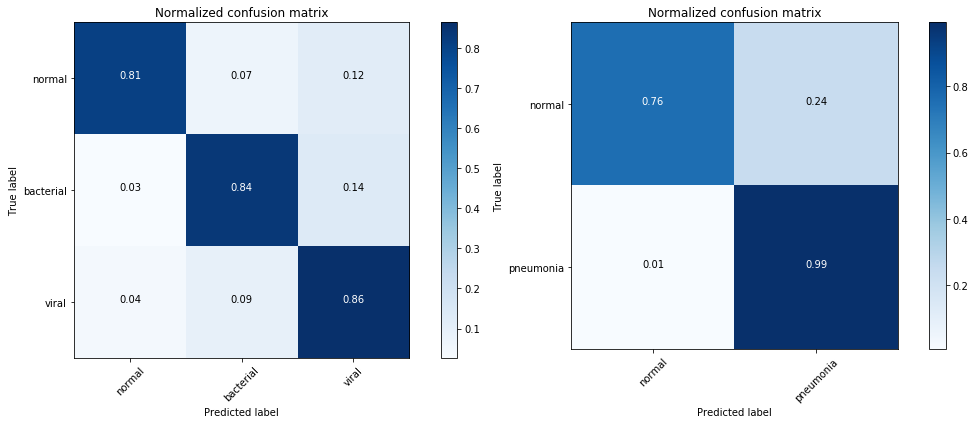
\includegraphics[scale=0.45]{combined-confusion.png}}
\caption{Normalized confusion matrix for (left) multi-class model and (right) binary-class model.}
\label{fig}
\end{figure*}

\begin{figure*}[htbp]
\centerline{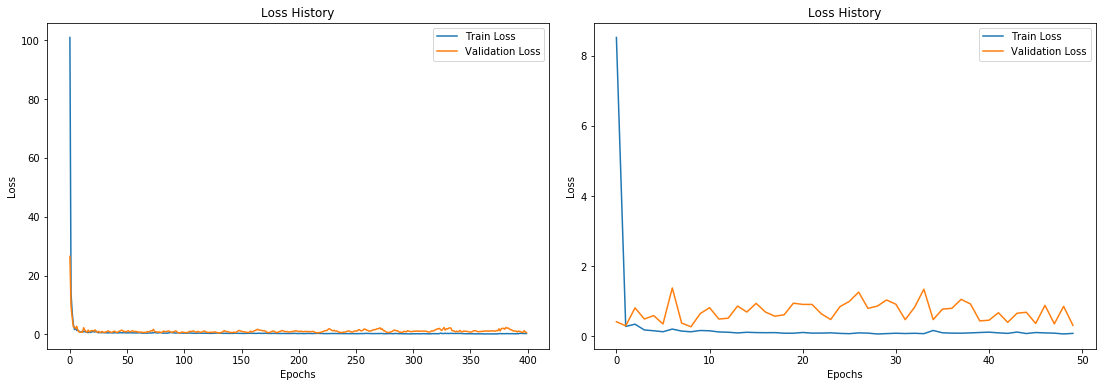
\includegraphics[scale=0.45]{combined-loss.png}}
\caption{Train and validation loss for (left) multi-class model and (right) binary-class model.}
\label{fig}
\end{figure*}

\section{Discussion}
As expected, our binary classifier performed better than our 3-classifier model because differences in features between viral and bacterial pneumonia images were very subtle. Our binary model performed similarly to Kermany et. al (2018) who used the same dataset and achieved 92.8\% with a sensitivity of 93.2\% and a specificity of 90.1\% for their pneumonia vs. normal model \cite{kermany2018identifying}. For a bacterial vs. viral pneumonia model, which we did not replicate, they achieved a test accuracy of 90.7\%, with a sensitivity of 88.6\% and a specificity of 90.9\% \cite{kermany2018identifying}. Our final best model results for the first binary model were slightly lower, and exact results were difficult to replicate because the large batch size of 1000 increased randomness across runs. Another factor is due to the data imbalance that we accounted for by under-sampling to the minimum number of images from training, validation, and testing sets. Kermany's test data set consisted of 234 normal images and 390 pneumonia images, while our test data sets had 74 for normal and 148 for pneumonia to account for imbalance.

Many configurations of the model were stuck with roughly 66\% accuracy because it was unable to predict any of the viral pneumonia correctly. The 3-class problem likely needed more data to allow the model to learn features that would better differentiate bacterial and viral pneumonia. 

While we did see small improvements in performances by using data augmentation, performance could have been increased if we had a greater variety of images since data augmentation could not generate completely new images. For instance, radiologists are provided with supplemental lateral view X-rays when making a diagnosis, however the dataset taken from Kaggle only contained frontal images. The patient’s health record is also often used as supplemental information that is taken into consideration to make the diagnosis. Predicting diagnoses based on a more comprehensive data set for each patient would be a more appropriate representation of clinical practices and may lead to better performance. 


\section{Conclusion}
We found that convolutional neural networks are effective at diagnosing normal and abnormal chest X-rays with high accuracy and precision, but can struggle with differentiating types of abnormal X-rays. We were able to replicate previous work on the same data set \cite{kermany2018identifying}. Future work involves looking at class activation maps to determine what features the model thinks are relevant. These maps could help us interpret the model's decisions, a useful feature in medical diagnosis, and could help determine why it confuses viral with bacterial pneumonia. This project has shown that transfer learning can used to apply large convolutional neural networks to chest X-rays. 
\section*{Acknowledgment}

Thanks to Dr. Paul Sajda PhD, Dr. Andrew Laine PhD, and Arunesh Mittal, for overseeing this project. 


\bibliographystyle{plainurl} 
\bibliography{references}
\newpage
\section{Appendix}
\begin{figure}[htbp]
\centerline{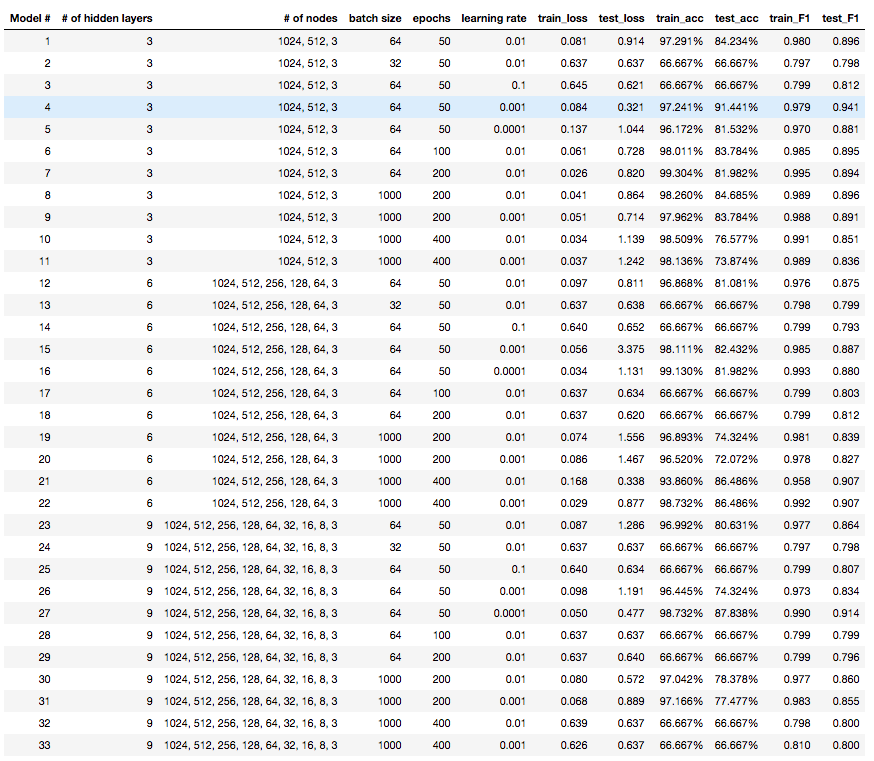
\includegraphics[scale=0.28]{bin_results.png}}
\caption{Hyperparameters tested for binary classifier (normal vs. pneumonia). The model with the highest accuracy is highlighted.}
\label{fig}
\end{figure}

\begin{figure}[htbp]
\centerline{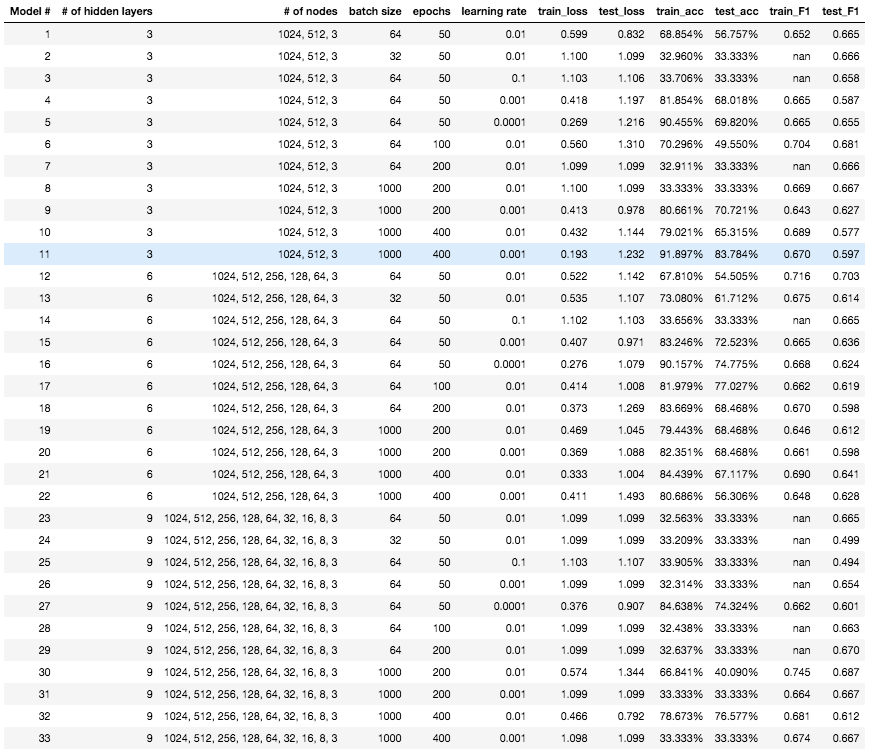
\includegraphics[scale=0.28]{multi_results.png}}
\caption{Hyperparameters tested for multi-classifier (normal vs. bacterial vs. viral pneumonia). The model with the highest accuracy is highlighted.}
\label{fig}
\end{figure}

\end{document}
